\documentclass[border=4pt]{standalone}
\usepackage{amssymb}
\usepackage{tikz}
\usetikzlibrary{arrows.meta,positioning,shapes.geometric,fit,calc,automata,trees}
\usepackage{float}
\usepackage{booktabs}
\usepackage{longtable}
\usepackage{array}
\usepackage[utf8]{inputenc}
\begin{document}

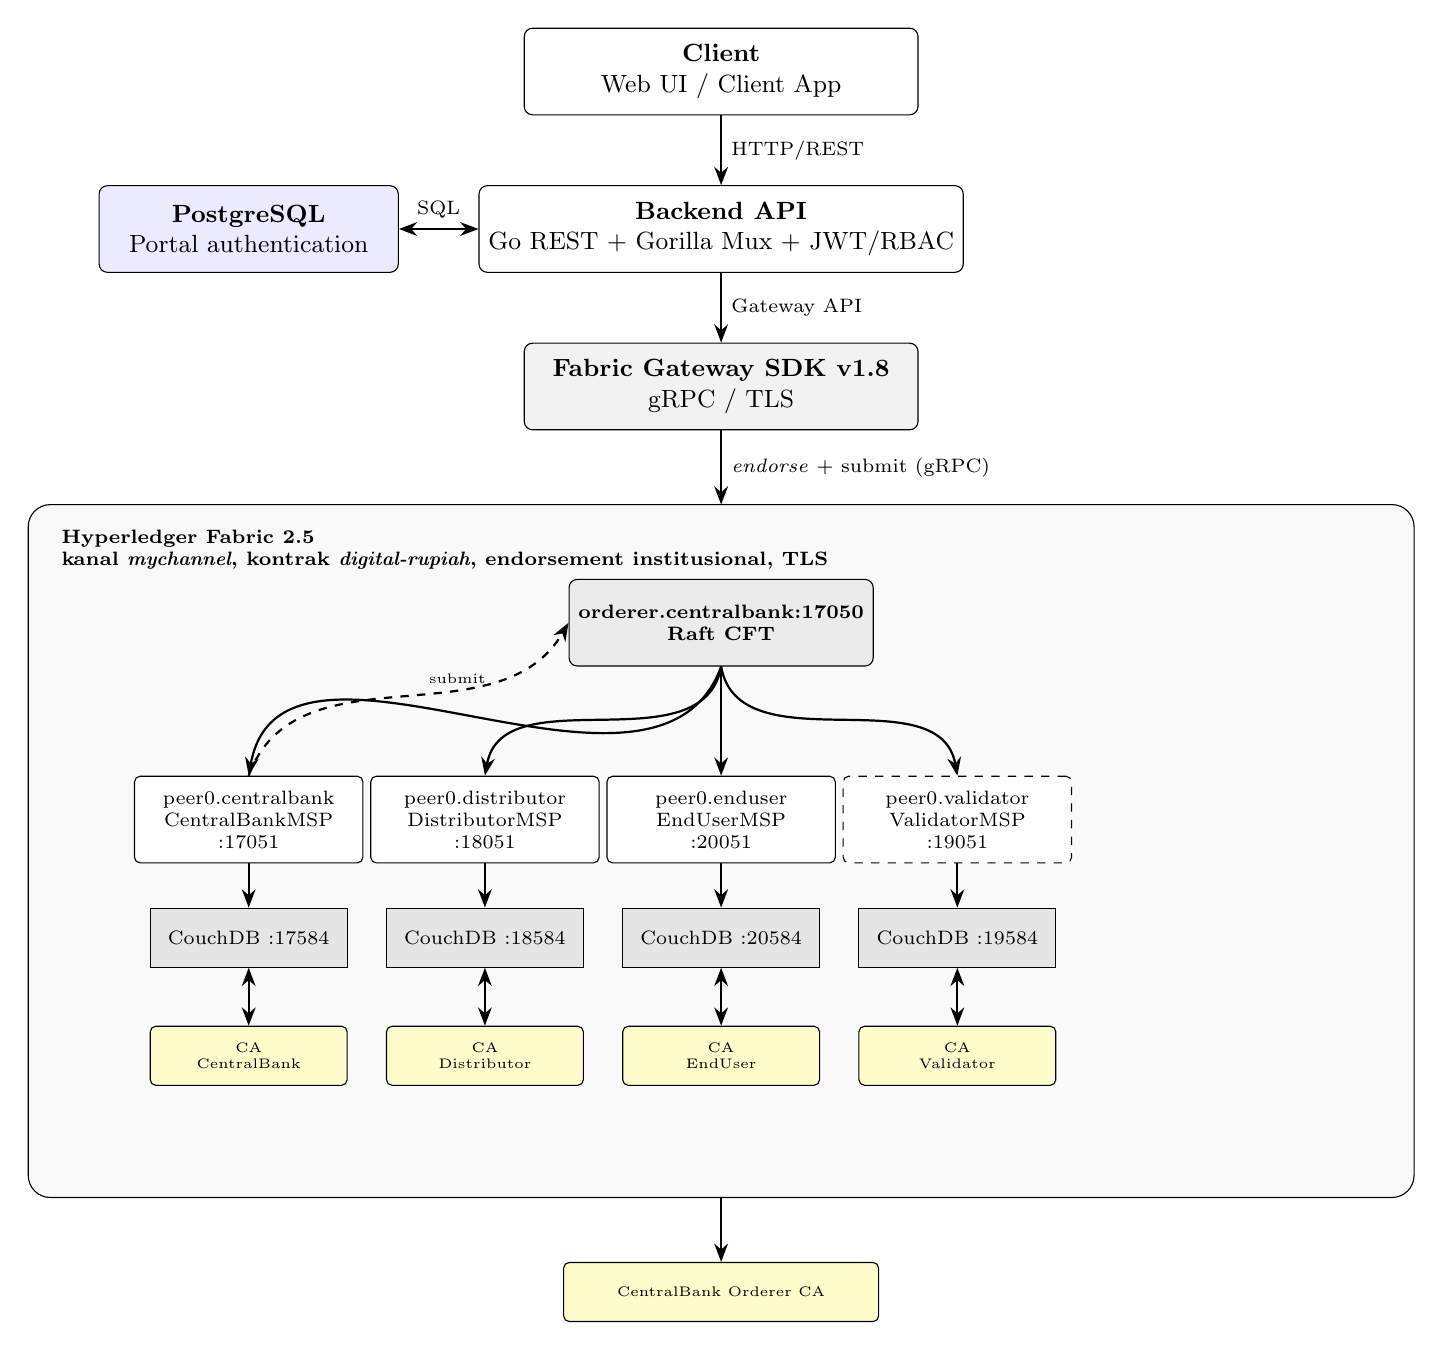
\begin{tikzpicture}[
  appbox/.style={draw=black, fill=white, rectangle, rounded corners=3pt,
    minimum width=5.0cm, minimum height=1.1cm, align=center, font=\small},
  gwbox/.style={draw=black, fill=black!5, rectangle, rounded corners=3pt,
    minimum width=5.0cm, minimum height=1.1cm, align=center, font=\small},
  pgbox/.style={draw=black, fill=blue!8, rectangle, rounded corners=3pt,
    minimum width=3.8cm, minimum height=1.1cm, align=center, font=\small},
  peer/.style={draw=black, fill=white, rectangle, rounded corners=2pt,
    minimum width=2.9cm, minimum height=1.1cm, align=center, font=\scriptsize},
  obsbox/.style={draw=black, dashed, fill=white, rectangle, rounded corners=2pt,
    minimum width=2.9cm, minimum height=1.1cm, align=center, font=\scriptsize},
  ordnode/.style={draw=black, fill=black!8, rectangle, rounded corners=3pt,
    minimum width=3.8cm, minimum height=1.1cm, align=center, font=\scriptsize\bfseries},
  cdb/.style={draw=black, fill=gray!20, rectangle,
    minimum width=2.5cm, minimum height=0.75cm, align=center, font=\scriptsize},
  cabox/.style={draw=black, fill=yellow!20, rectangle, rounded corners=2pt,
    minimum width=2.5cm, minimum height=0.75cm, align=center, font=\tiny},
  ar/.style={-{Stealth}, thick},
  bar/.style={{Stealth}-{Stealth}, thick},
  lbl/.style={font=\scriptsize, midway},
]

%── Lapisan Aplikasi ──────────────────────────────────────────────────────────

\node[appbox] (fe) at (6.0, 16.5) {\textbf{Client}\\Web UI / Client App};
\node[appbox] (be) at (6.0, 14.5) {\textbf{Backend API}\\Go REST + Gorilla Mux + JWT/RBAC};
\node[pgbox]  (pg) at (0.0, 14.5) {\textbf{PostgreSQL}\\Portal authentication};
\node[gwbox]  (gw) at (6.0, 12.5) {\textbf{Fabric Gateway SDK v1.8}\\gRPC / TLS};

\draw[ar]  (fe.south) -- (be.north)  node[lbl, right]{HTTP/REST};
\draw[bar] (be.west)  -- (pg.east)   node[lbl, above]{SQL};
\draw[ar]  (be.south) -- (gw.north)  node[lbl, right]{Gateway API};

%── Jaringan Hyperledger Fabric ───────────────────────────────────────────────
% Latar belakang kotak digambar PERTAMA agar node internal tampak di atasnya

\fill[rounded corners=8pt, gray!5]  (-2.8, 2.2) rectangle (14.8, 11.0);
\draw[rounded corners=8pt, black]   (-2.8, 2.2) rectangle (14.8, 11.0);
\node[font=\scriptsize\bfseries, anchor=north west, align=left] at (-2.5, 10.8)
  {\textbf{Hyperledger Fabric 2.5}\\
   kanal \textit{mychannel}, kontrak \textit{digital-rupiah}, endorsement institusional, TLS};

% Panah dari Gateway ke batas atas kotak jaringan
\draw[ar] (gw.south) -- (6.0, 11.0)
  node[lbl, right]{\textit{endorse} + submit (gRPC)};

%── Orderer ───────────────────────────────────────────────────────────────────

\node[ordnode] (ord) at (6.0, 9.5)
  {orderer.centralbank:17050\\Raft CFT};

%── Empat Peer ─────────────────────────────────────────────────────────────────

\node[peer]   (pbi)  at (0.0,  7.0)
  {peer0.centralbank\\CentralBankMSP\\:17051};
\node[peer]   (pdist) at (3.0,  7.0)
  {peer0.distributor\\DistributorMSP\\:18051};
\node[peer]   (pend) at (6.0,  7.0)
  {peer0.enduser\\EndUserMSP\\:20051};
\node[obsbox] (pval) at (9.0,  7.0)
  {peer0.validator\\ValidatorMSP\\:19051};

% Orderer → semua peer (pengiriman blok)
\draw[ar] (ord.south) to[out=-110,in=80] (pbi.north);
\draw[ar] (ord.south) to[out=-100,in=80] (pdist.north);
\draw[ar] (ord.south) -- (pend.north);
\draw[ar] (ord.south) to[out=-80,in=100]  (pval.north);

% peer0.bi → orderer (endorsement submit)
\draw[ar, dashed] (pbi.north) to[out=70,in=-120]
  node[near end, left, font=\tiny]{submit} (ord.west);

%── CouchDB ───────────────────────────────────────────────────────────────────

\node[cdb] (cbi)   at (0.0,  5.5) {CouchDB :17584};
\node[cdb] (cdist) at (3.0,  5.5) {CouchDB :18584};
\node[cdb] (cend)  at (6.0,  5.5) {CouchDB :20584};
\node[cdb] (cval)  at (9.0,  5.5) {CouchDB :19584};

\draw[ar] (pbi)   -- (cbi);
\draw[ar] (pdist) -- (cdist);
\draw[ar] (pend)  -- (cend);
\draw[ar] (pval)  -- (cval);

%── CA per Organisasi ─────────────────────────────────────────────────────────

\node[cabox] (cabi)   at (0.0,  4.0) {CA\\CentralBank};
\node[cabox] (cadist) at (3.0,  4.0) {CA\\Distributor};
\node[cabox] (caend)  at (6.0,  4.0) {CA\\EndUser};
\node[cabox] (caval)  at (9.0,  4.0) {CA\\Validator};

\draw[bar] (cabi)   -- (cbi);
\draw[bar] (cadist) -- (cdist);
\draw[bar] (caend)  -- (cend);
\draw[bar] (caval)  -- (cval);

%── Orderer CA (di bawah kotak jaringan) ─────────────────────────────────────

\node[cabox, minimum width=4.0cm] (caord) at (6.0, 1.0)
  {CentralBank Orderer CA};
\draw[ar] (6.0, 2.2) -- (caord.north);

\end{tikzpicture}%

\end{document}
